\documentclass[border=2pt]{standalone}
\usepackage{tikz}
\begin{document}
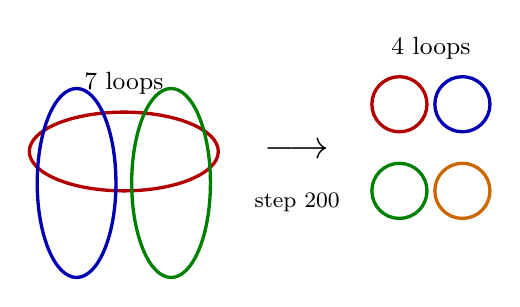
\begin{tikzpicture}
  % Three interlocked rings (Borromean-style schematic)
  \draw[very thick, red!70!black] (0,0) ellipse (1.2 and 0.5);
  \draw[very thick, blue!70!black] (-0.6,-0.4) ellipse (0.5 and 1.2);
  \draw[very thick, green!50!black] (0.6,-0.4) ellipse (0.5 and 1.2);
  % Labels
  \node[above] at (0,0.6) {\small 7 loops};
  \node[font=\Large] at (2.2,0) {$\longrightarrow$};
  % Right side: 4 separate loops
  \draw[very thick, red!70!black] (3.5,0.6) circle (0.35);
  \draw[very thick, blue!70!black] (4.3,0.6) circle (0.35);
  \draw[very thick, green!50!black] (3.5,-0.5) circle (0.35);
  \draw[very thick, orange!80!black] (4.3,-0.5) circle (0.35);
  \node[above] at (3.9,1.05) {\small 4 loops};
  % Step label
  \node[below, font=\footnotesize] at (2.2,-0.4) {step 200};
\end{tikzpicture}
\end{document}
